% Copyright 2004 by Till Tantau <tantau@users.sourceforge.net>.
%
% In principle, this file can be redistributed and/or modified under
% the terms of the GNU Public License, version 2.
%
% However, this file is supposed to be a template to be modified
% for your own needs. For this reason, if you use this file as a
% template and not specifically distribute it as part of a another
% package/program, I grant the extra permission to freely copy and
% modify this file as you see fit and even to delete this copyright
% notice. 
\documentclass{beamer}

\usepackage{graphicx}
 \graphicspath{{./images/}}
\usepackage{pgf-pie}
\usepackage{amsmath}
\usepackage{wrapfig}

% There are many different themes available for Beamer. A comprehensive
% list with examples is given here:
% http://deic.uab.es/~iblanes/beamer_gallery/index_by_theme.html
% You can uncomment the themes below if you would like to use a different
% one:
%\usetheme{AnnArbor}
%\usetheme{Antibes}
%\usetheme{Bergen}
%\usetheme{Berkeley}
%\usetheme{Berlin}
%\usetheme{Boadilla}
%\usetheme{boxes}
%\usetheme{CambridgeUS}
%\usetheme{Copenhagen}
%\usetheme{Darmstadt}
%\usetheme{default}
%\usetheme{Frankfurt}
%\usetheme{Goettingen}
%\usetheme{Hannover}
%\usetheme{Ilmenau}
%\usetheme{JuanLesPins}
%\usetheme{Luebeck}
\usetheme{Madrid}
%\usetheme{Malmoe}
%\usetheme{Marburg}
%\usetheme{Montpellier}
%\usetheme{PaloAlto}
%\usetheme{Pittsburgh}
%\usetheme{Rochester}
%\usetheme{Singapore}
%\usetheme{Szeged}
%\usetheme{Warsaw}

% Change base colour beamer@blendedblue (originally RGB: 0.2,0.2,0.7)
\colorlet{beamer@blendedblue}{red!40!black}


\title{Diabetic Retinopathy Classification and Interpretation using Deep Learning Techniques}

% A subtitle is optional and this may be deleted
%\subtitle{}

\author{Jordi de la Torre\inst{1} \\supervised by:\\ A\"ida Valls\inst{1} and Dom\`enec Puig\inst{1}} %\and S.~Another\inst{2}}
% - Give the names in the same order as the appear in the paper.
% - Use the \inst{?} command only if the authors have different
%   affiliation.

\institute[Universitat Rovira i Virgili] % (optional, but mostly needed)
{
  \inst{1}%
  Department d'Enginyeria Inform\`atica i Matem\`atiques\\
  Escola T\`ecnica Superior d'Enginyeria\\
  Universitat Rovira i Virgili}
  %\and
  %\inst{2}%
  %Department of Theoretical Philosophy\\
  %University of Elsewhere}
% - Use the \inst command only if there are several affiliations.
% - Keep it simple, no one is interested in your street address.

\date{\today}
% - Either use conference name or its abbreviation.
% - Not really informative to the audience, more for people (including
%   yourself) who are reading the slides online

\subject{Computer Science}
% This is only inserted into the PDF information catalog. Can be left
% out. 

% If you have a file called "university-logo-filename.xxx", where xxx
% is a graphic format that can be processed by latex or pdflatex,
% resp., then you can add a logo as follows:

\pgfdeclareimage[height=0.3cm]{itaka}{itaka.png}
\pgfdeclareimage[height=0.3cm]{rivi}{rivi.png}
\pgfdeclareimage[height=0.5cm]{urv}{urv.jpg}
\logo{\pgfuseimage{itaka}\pgfuseimage{rivi}\pgfuseimage{urv}}

% Delete this, if you do not want the table of contents to pop up at
% the beginning of each subsection:
\AtBeginSubsection[]
{
  \begin{frame}<beamer>{Outline}
    \tableofcontents[currentsection,currentsubsection]
  \end{frame}
}

% Let's get started
\begin{document}

\begin{frame}
  \titlepage
\end{frame}

\begin{frame}{Outline}
  \tableofcontents
  % You might wish to add the option [pausesections]
\end{frame}

% Section and subsections will appear in the presentation overview
% and table of contents.
\section{Research line description}

\subsection{Motivation}

\begin{frame}{The motivation of the research}{Diabetic Retinopathy}
\begin{columns}
	\begin{column}{0.5\textwidth}
		\begin{itemize}
	  	 	\item {Diabetic Retinopathy (DR) is a leading disabling chronic disease.}
	  	 	\item {Main cause of blindness and visual impairment in developed countries for diabetic patients.}
	  	 	\item{Diagnostic automation can help the physicians to improve the quality of their diagnostics and reduce the cost associated with it.}
	  	\end{itemize}	
	\end{column}
	\begin{column}{0.5\textwidth}  %%<--- here
		\begin{figure}[p]
			\centering
			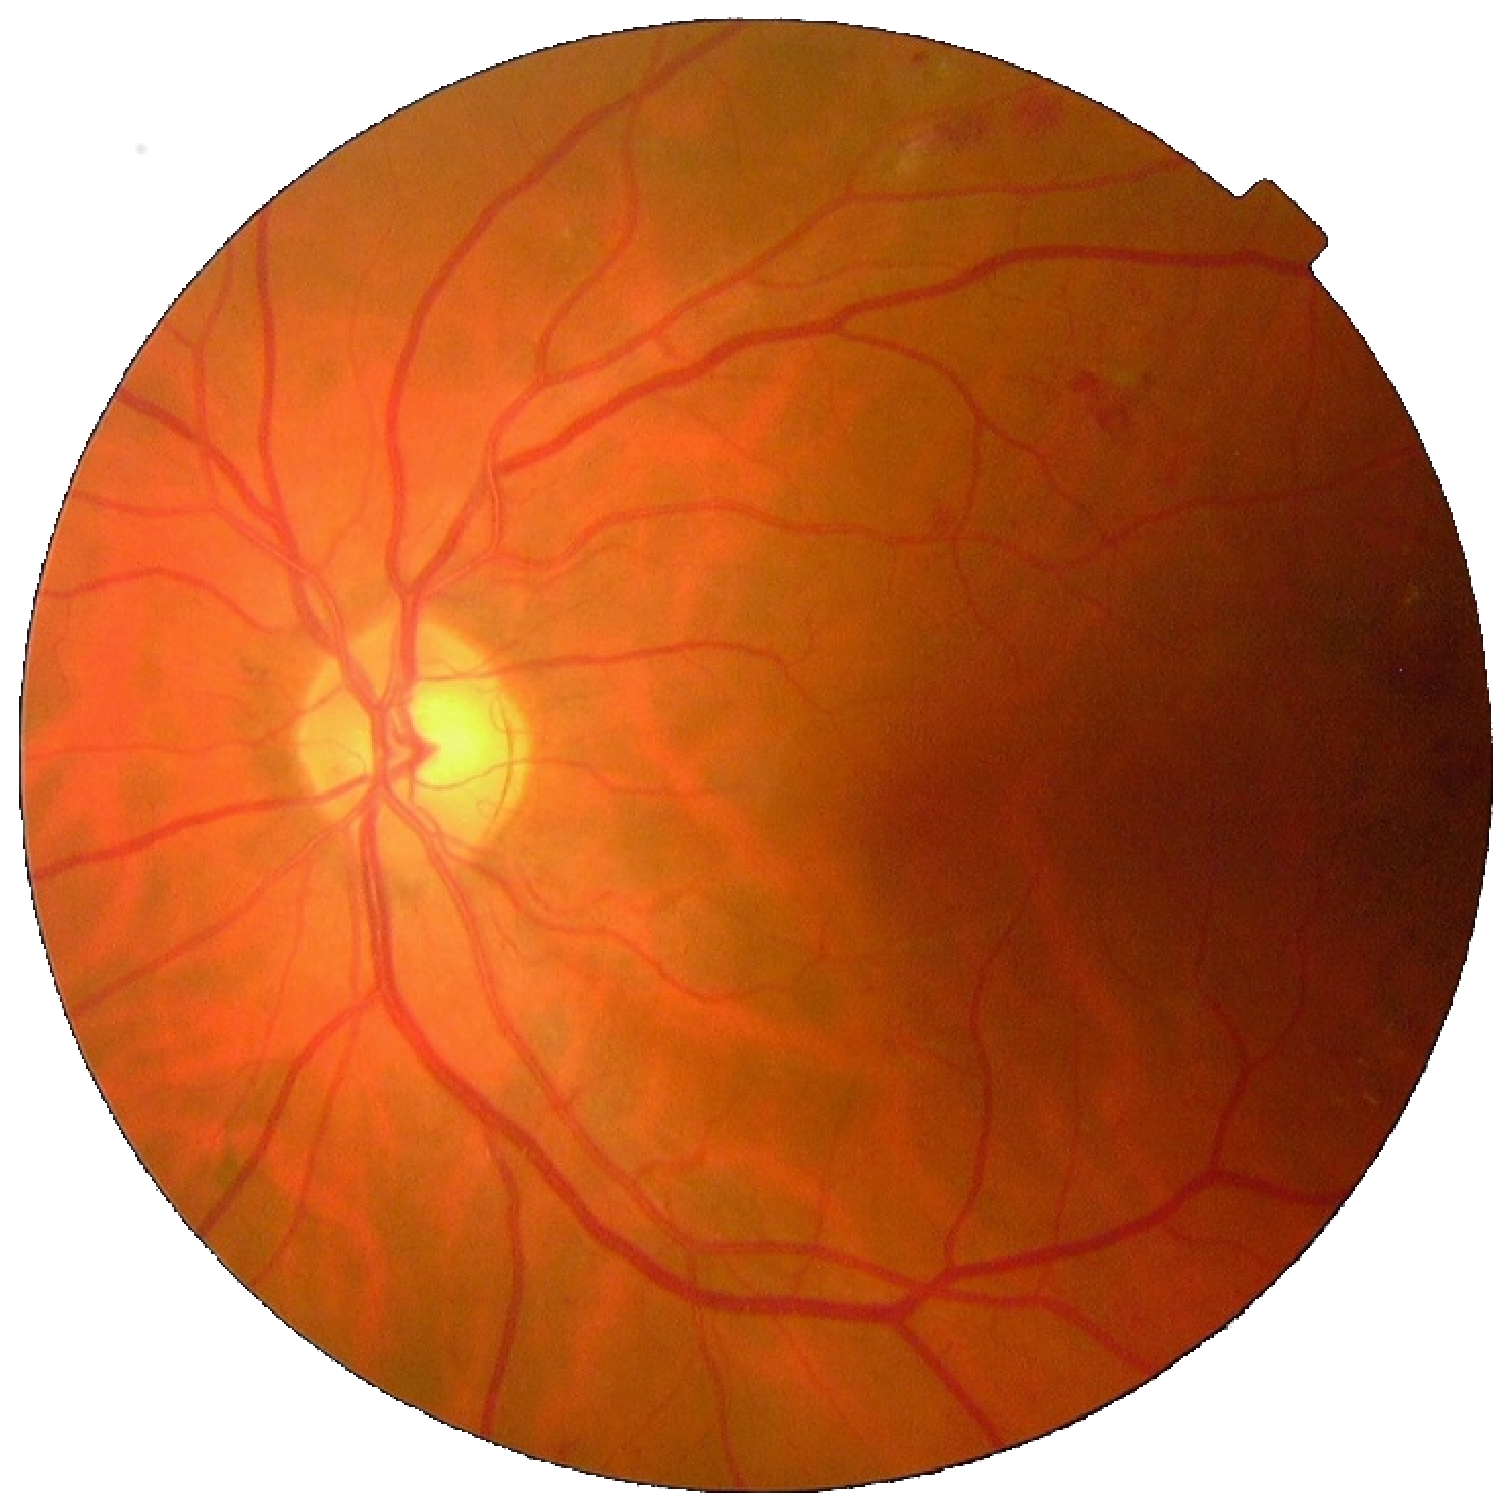
\includegraphics[width=0.5\textwidth]{retine.eps}
			\caption{Image taken with a non-mydriatic fundus camera.}
		\end{figure}
	\end{column}
\end{columns}

\end{frame}

\begin{frame}{The problem to solve}{Diabetic Retinopathy Grade Classification}
	\begin{itemize}
		\item {Classification of retine images into 5 different categories of increasing disease grade.}
		\item {It is a standardized classification defined by ophthalmologists (depending on the number and type of retinal lesions present on the image).}
	\end{itemize}
	\begin{figure}[p]
		\includegraphics[width=0.9\textwidth]{classes.eps}
		\caption{Five samples of increasing grade. From left to right: 0, no apparent DR; 1, mild non-proliferative (NPDR); 2, moderate NPDR; 3, severe NPDR and 4, proliferative DR}
	\end{figure}	
\end{frame}

\subsection{Objectives}

\begin{frame}{Objectives of the research}
	\begin{itemize}
		\item {
			Design a method for extracting the statistical regularities present in the data that are important for the classification with the minimum human intervention.
		}
		% You can also specify when the content should appear
		% by using <n->:
		\item {The model should learn alone the important features, not requiring the Computer Scientist to become an expert on the problem that is solving, but only requiring knowledge about the Machine Learning algorithms.}
		\item {The model should be self explainable.}
	\end{itemize}
\end{frame}

\subsection{Mathematical formalization}
% You can reveal the parts of a slide one at a time
% with the \pause command:
\begin{frame}{Mathematical formalization}
  \begin{itemize}
  \item {   
    Find a function f: $\mathbb{R}^{CxHxW} 
    \mapsto \mathbb{R}^{n}$ that maximizes a objective function (where $CxHxW \gg n$). \alert{Optimization}.
  }
  % You can also specify when the content should appear
  % by using <n->:
  \item {
  	Images are high dimensional objects with highly correlated local points.
    Function proven to exploit this characteristics: a \alert{deep convolutional neural network}.
  }
  \item {
    \alert{Objective function} in neural network argot called \alert{cost function}.
  }
  % or you can use the \uncover command to reveal general
  % content (not just \items):
  \item {
    Standardized cost function for classification: \alert{logarithmic loss} (log-loss).
  }
  \item {
  	Evaluation metric: \alert{quadratic weighed kappa} (QWK).
  }
  \end{itemize}
\end{frame}

\subsection{The data}

\begin{frame}{The dataset}{Whole dataset of near 85,000 images, 10x10}
	\includegraphics[width=1.0\textwidth]{mosaic-85000-10x10.png}	
\end{frame}

\begin{frame}{The dataset}{10,000 random images, 25x25}
	\includegraphics[width=1.0\textwidth]{mosaic-10000-25x25.png}	
\end{frame}

\begin{frame}{The dataset}{2,000 random images, 50x50}
	
\includegraphics[width=1.0\textwidth]{mosaic-2000-50x50.png}	
\end{frame}

\begin{frame}{The dataset}{500 random images, 100x100}
	
\includegraphics[width=1.0\textwidth]{mosaic-500-100x100.png}	
\end{frame}


\begin{frame}{The dataset}{Exploratory data analysis}
	\begin{columns}
		\begin{column}{0.5\textwidth}
			\begin{figure}[p]
				\resizebox{.61\textwidth}{!}{
					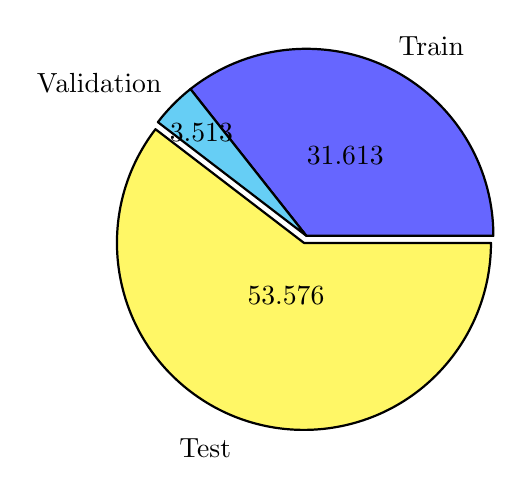
\begin{tikzpicture}[scale = 0.95]
					\pie[sum=auto , after  number=, radius = 2.5, explode={0, 0, 0.1}]{31.613/Train, 3.513/Validation,  53.576/Test}
					\end{tikzpicture}
				}
				\caption{Dataset conformation}
			\end{figure}	
		\end{column}
		\begin{column}{0.4\textwidth}  %%<--- here
			\begin{figure}[p]
				\resizebox{.95\textwidth}{!}{
					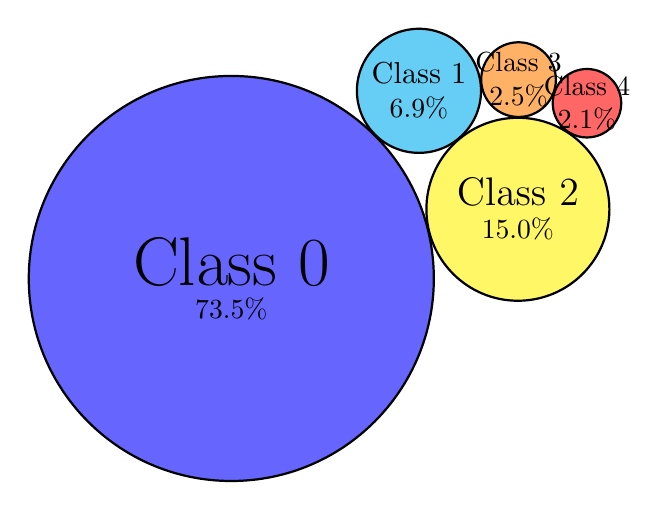
\begin{tikzpicture}[scale=0.10]
					\pie[cloud, text=inside,scale font, radius=30]
					{
						73.5/Class 0,
						6.9/Class 1,
						15.0/Class 2,
						2.5/Class 3,
						2.1/Class 4
					}
					\end{tikzpicture}
				}
				\caption{Dataset class percentage}
			\end{figure}
		\end{column}
	\end{columns}	
	\begin{itemize}
		\item Images with differing sizes, illumination conditions, quality.\\ 
		\item For every patient: right and left eye images available.
	\end{itemize}
\end{frame}

\begin{frame}{Data pre-processing}{Minimal}
	Minimal data preprocessing applied (optimization of hardware resources, deep learning optimization methods are computer intensive tasks): 
	\begin{itemize}
		\item Remove borders
		\item Standardization of the image size (downsizing: 128, 256, 512, etc.) depending on the model requirements.
	\end{itemize}
	
	\begin{columns}
		\begin{column}{0.5\textwidth}
			\begin{figure}[p]
				\resizebox{.74\textwidth}{!}{
					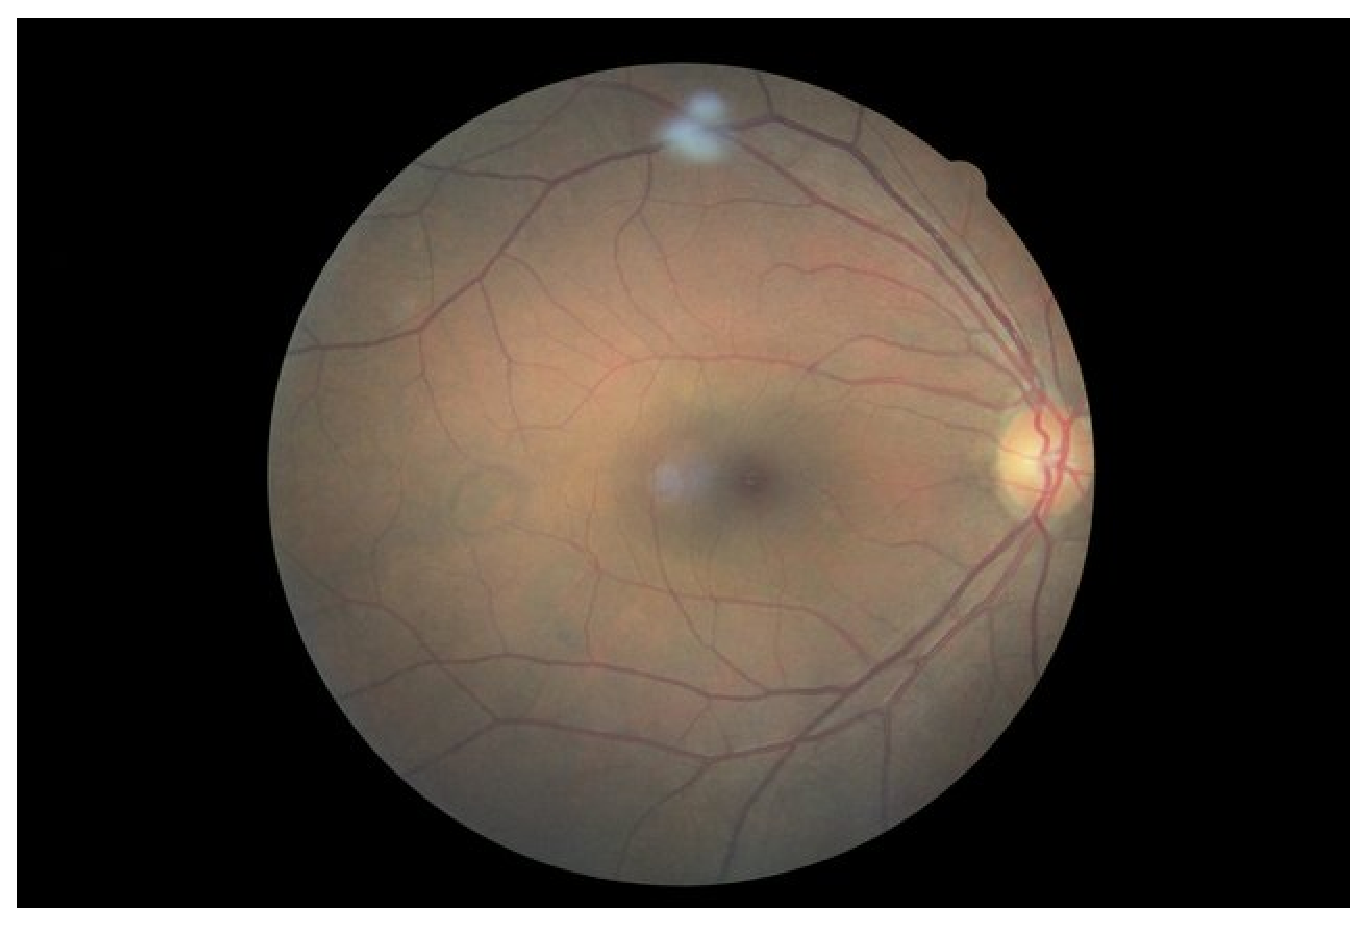
\includegraphics[width=1.0\textwidth]{61_right-4752x3168.eps}
				}
				\caption{Original 4752x3168 pixels}
			\end{figure}	
		\end{column}
		\begin{column}{0.31\textwidth}  %%<--- here
			\begin{figure}[p]
				\resizebox{.74\textwidth}{!}{
					\includegraphics[width=1.0\textwidth]{61_right-4752x3168-trimmed.eps}
				}
				\caption{Preprocessed: trimmed + resized}
			\end{figure}
		\end{column}
	\end{columns}	
\end{frame}

\section{Publications}

\subsection{A deep learning model for DR image classification (CCAI 2016)}

\begin{frame}{A deep learning model for DR image classification}{Key points of this work}
	\begin{columns}
	\begin{column}{0.7\textwidth}
		\begin{itemize}
			\item Data augmentation techniques were necessary to balance the classes and to increment the generalization capabilities of the model (brightness,contrast, rotations).
			\item Due to hardware limitations only a part of the input was feeded to the network (about 71\% of the useful information), requiring various evaluations and ensembling on test time to increase performance.
			\item Probabilistic combination of results of both eyes (Bayes rule) helps improve further performance.
		\end{itemize}
	\end{column}
	\begin{column}{0.3\textwidth}
			\begin{figure}[p]
				\resizebox{.75\textwidth}{!}{
					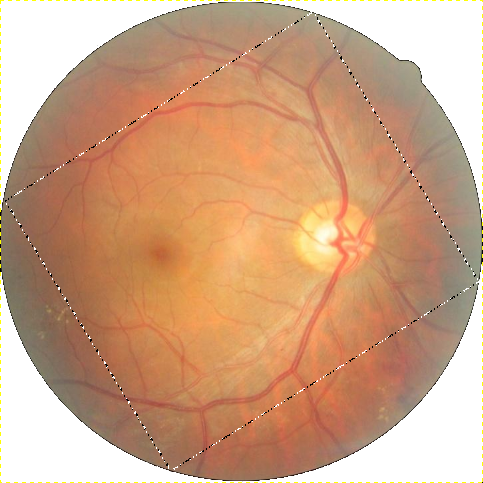
\includegraphics[width=1.0\textwidth]{input-ccia2016-paper.png}
				}
				\caption{Input data selection}
			\end{figure}
	\end{column}
	\end{columns}
\end{frame}

\begin{frame}{A deep learning model for DR image classification}{Model and training overview (CCIA 2016)}	
	\begin{columns}
		\begin{column}{0.2\textwidth}
			\centering
			\begin{figure}[p]
			\resizebox{.45\textwidth}{!}{
				\includegraphics[width=1.0\textwidth]{nnarch-crop.pdf}	
			}
			\caption{Model}
			\end{figure}
		\end{column}
		\begin{column}{0.5\textwidth}
			\begin{figure}[p]
				\resizebox{.3\textwidth}{!}{
					\includegraphics[width=1.0\textwidth]{training-crop.pdf}
				}
				\caption{Training}
			\end{figure}	
		\end{column}
		\begin{column}{0.3\textwidth}  %%<--- here
			\begin{figure}[p]
				\resizebox{.9\textwidth}{!}{
					\includegraphics[width=1.0\textwidth]{testing-crop.pdf}				
				}
				\caption{Evaluation}
			\end{figure}
			\begin{figure}[p]
				\resizebox{.9\textwidth}{!}{
					\includegraphics[width=1.0\textwidth]{combination-crop.pdf}				
				}
				\caption{Combination}
			\end{figure}
		\end{column}
	\end{columns}	
\end{frame}

\begin{frame}{A deep learning model for DR image classification}{Results}	
\begin{table}[h!]
	\centering
	\begin{tabular}{c c c c} 
		\hline		
		Layers & Input size & $\kappa_{test, alone}$ & $\kappa_{test, combined}$\\ [0.5ex] 
		\hline\hline
		12 & (3,128,128) & 0.488 & 0.577\\ 
		14 & (3,256,256) & 0.636 & 0.660\\ 
		16 & (3,384,384) & 0.668 & 0.730 \\ 
		16 & (3,512,512) & 0.725 & 0.769\\ 
		\hline
	\end{tabular}
	\caption{Comparison of results obtained with and without probabilistic combination}
	\label{table-results2}
\end{table}
\end{frame}

\subsection{QWK: A new loss function for ordinal regression (PRL)}


\begin{frame}{QWK: A new loss function for ordinal regression}{Mathematical summary of the paper (Pattern Recognition Letters, 2017)}	
	Model function: $p = f(I) \quad where \quad I \in \mathbb{R}^{CxHxW}, \quad p \in \mathbb{R}^n$
	\begin{columns}
		\begin{column}{0.5\textwidth}
			\\
			\alert{Log-loss optimization:}
			\begin{equation*}
				min \quad C = \sum_{i=1}^{BS} \sum_{j=1}^{n} t_{i,j} log(p_{i,j})
			\end{equation*}			
			First order derivative:\\
			\begin{equation*}
				\frac{\partial C}{\partial p_{i,j}} = \frac{t_{i,j}}{p_{i,j}}
			\end{equation*}							
		\end{column}
		\begin{column}{0.5\textwidth}  %%<--- here
			\\
			\alert{QWK-loss optimization:}\\
			\begin{equation*}
			max \quad \kappa = \frac{\sum_{i,j} \omega_{i,j}O_{i,j}}{\sum_{i,j} \omega_{i,j} E_{i,j}} 
			\end{equation*}		
			\begin{equation*}
			min \quad C = log(1 - \kappa), \quad \omega_{i,j} = \frac{(i-j)^2}{(n-1)^2}
			\end{equation*}		
				
			First order derivative (check paper for details of the derivation).			
		\end{column}
	\end{columns}	
\end{frame}

\begin{frame}{QWK: A new loss function for ordinal regression}{Pattern Recognition Letters, 2017}	
	\begin{itemize}
		\item  Three different multi-class classification problems using as evaluation metric QWK were trained using QWK-loss and log-loss.
		\item Different neural networks were tested: a linear classifier, a shallow neural network of 2-3 layers and a deep neural network of up to 16 layers.
		\item Optimizing QWK reported in all the models and problems increases of performance in the test set of about 5 to 10\% over the conventional training method.
\end{itemize}	
\end{frame}

\begin{frame}{QWK: A new loss function for ordinal regression}{Results}	
	\begin{columns}
		\begin{column}{0.5\textwidth}
			\begin{figure}[p]
				\resizebox{.5\textwidth}{!}{
					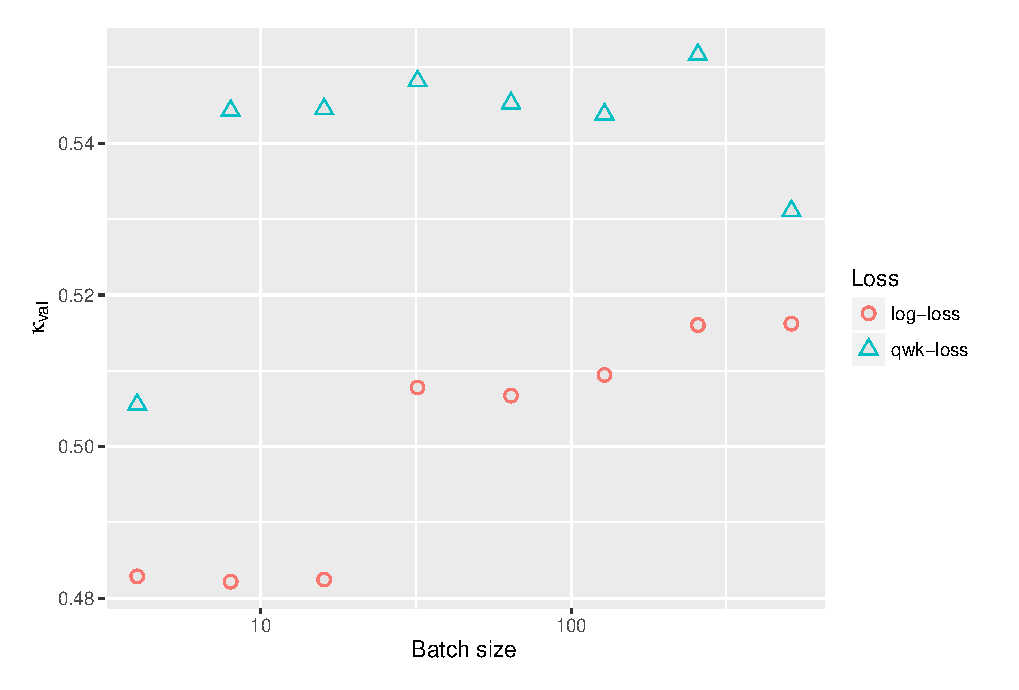
\includegraphics[width=1.0\textwidth]{crowdflower-results.eps}
				}
				\caption{LC for search results relevance}
			\end{figure}
			\begin{figure}[p]
				\resizebox{.5\textwidth}{!}{
					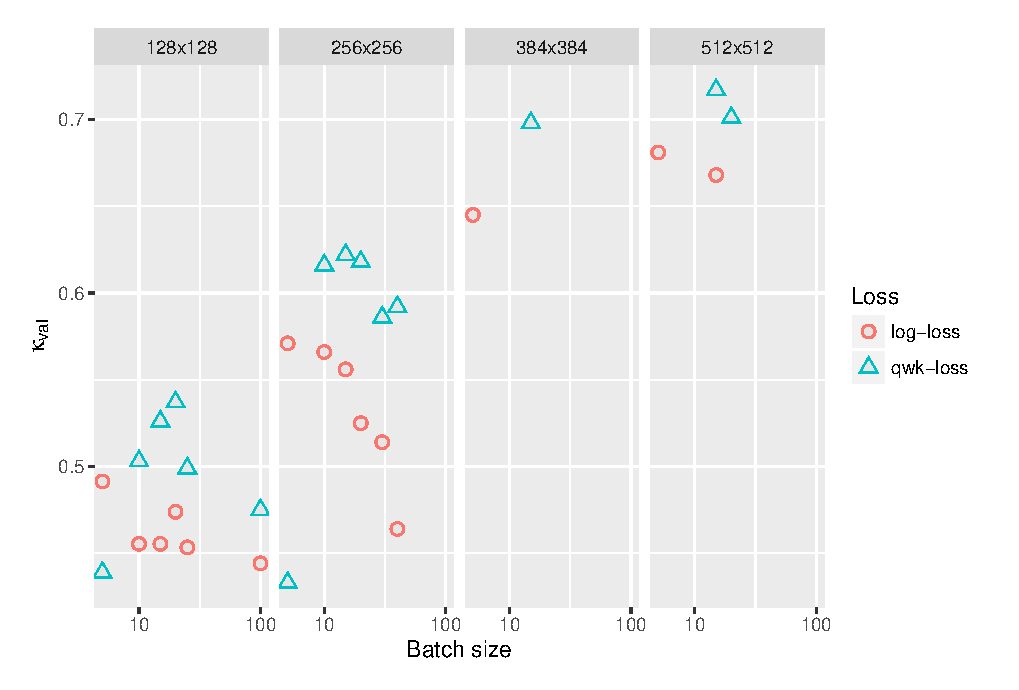
\includegraphics[width=1.0\textwidth]{retine-results.eps}
				}
				\caption{DCNN for DR classification}
			\end{figure}			
		\end{column}
		\begin{column}{0.5\textwidth}  %%<--- here
			\begin{figure}[p]
				\resizebox{.5\textwidth}{!}{
					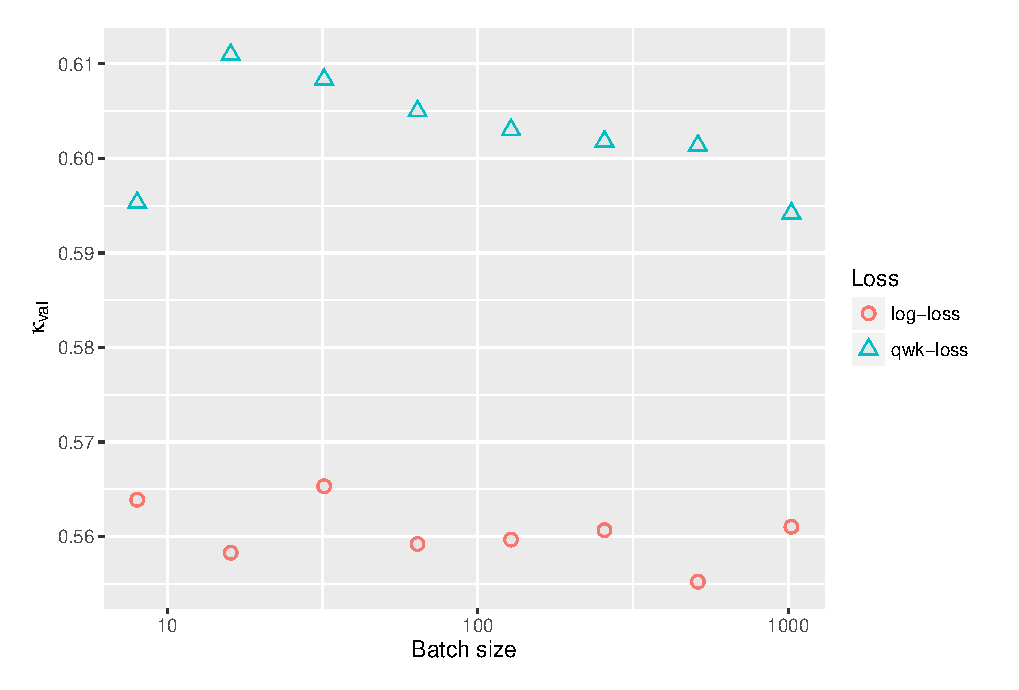
\includegraphics[width=1.0\textwidth]{prudential-results.eps}				
				}
				\caption{SNN insurance assessment}
			\end{figure}
			\begin{figure}[p]
				\resizebox{.5\textwidth}{!}{
					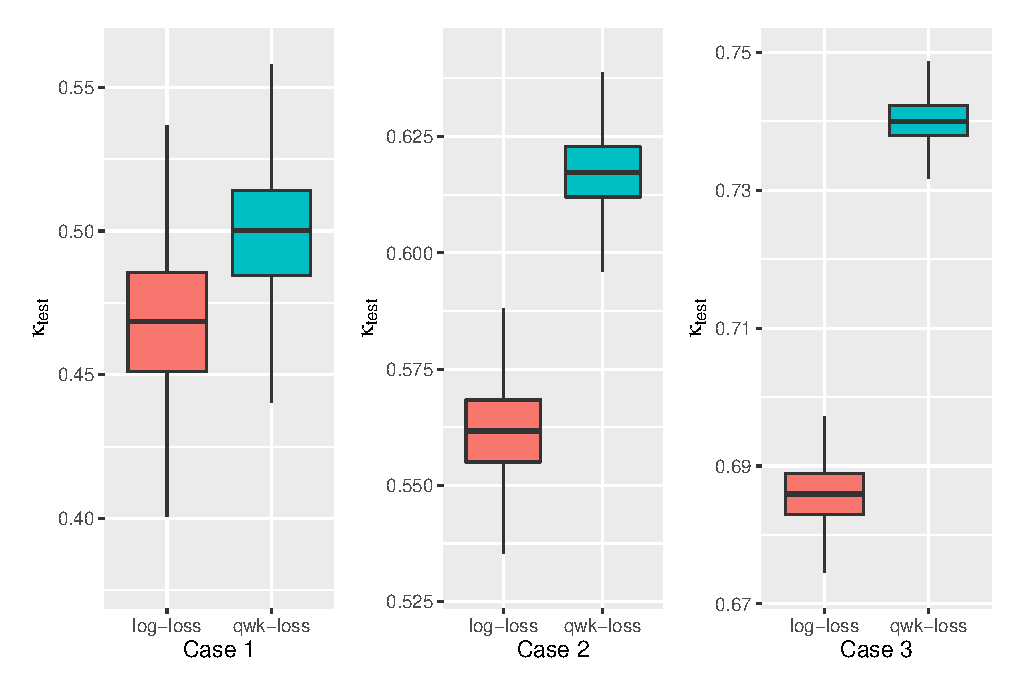
\includegraphics[width=1.0\textwidth]{boxplots.eps}				
				}
				\caption{Confidence intervals (test)}
			\end{figure}
		\end{column}
	\end{columns}	
\end{frame}

\section{Present and future work}
\begin{frame}{Present and future work}{Self explanaible models}	
	\begin{itemize}
		\item  Deep learning is able to generate models that work very well when trained in a supervised way in the presence of lots of data (thousands of samples per class).
		\item The drawback of these models is its lack of interpretability. Most of the time act as black boxes.
		\item Excellent classification performance is a must in medical diagnosis but not enough. Explanation of the reasons behind a result are very important for diagnosis confirmation.
		\item We are working on improving the interpretability of deep learning in general and of our models in particular.
	\end{itemize}	
\end{frame}



% Placing a * after \section means it will not show in the
% outline or table of contents.
\section*{Summary}

\begin{frame}{Summary}
  \begin{itemize}
  \item
    We designed a end to end model for the diagnosis of diabetic retinopathy disease reporting statistical results on the evaluation metric QWK better than human experts.
  \item Our prediction models are reporting right now QWK values in test set of about 0.844 (Human expert considered with results $QWK\ge0.80$)    
  \item
    We proposed the use of a new loss function for the optimization in ordinal regression of neural network based models that report increases of performance of more than a 5\%.
  \item
    We are working on the interpretability of deep learning models.
  \end{itemize}
\end{frame}

\begin{frame}{End}
\centering
\huge Thank you.
\end{frame}

\end{document}


